\section{Methodology}
\label{sec:methodology}

We first specify the policy family whose information weight will be calibrated to a sensing target. The EFE connection identifies one member of that family under explicit reward and information-unit conventions. It does not establish reward optimality.

\subsection{The $\rho$-POMDP Framework}

A $\rho$-POMDP adds a belief-dependent utility $\rho:\Delta(S)\times\mathcal{A}\to\mathbb{R}$ to task reward, giving the objective
\begin{equation}
\pi^* = \arg\max_\pi \mathbb{E}_\pi\!\left[\sum_{t=0}^{H}\gamma^t\big(R(s_t,a_t)+\rho(b_t,a_t)\big)\right].
\end{equation}
Here $S$ is the finite hidden-state space, $\mathcal A$ the action set, $b_t\in\Delta(S)$ the Bayesian belief, $H$ the planning horizon, and $\gamma$ the discount factor. The expectation runs over the initial state, state transitions, observations, and resulting belief updates under policy $\pi$. Setting $\rho=0$ recovers a standard POMDP. Choosing information gain as $\rho$ explicitly rewards uncertainty reduction. The equivalence below concerns $\gamma=1$.

In the observe-then-commit class, $\mathcal A$ partitions into observation actions $\mathcal A_{\mathrm{obs}}$, which leave the hidden state fixed and update the belief at known cost, and terminal commit actions $\mathcal A_{\mathrm{com}}$, which yield state-dependent reward and emit no observation. Rewards are not observations: beliefs are conditioned on observation symbols alone. Each episode consists of observations followed by one commit. This structure isolates the information-weight question and permits analytic thresholds and near-optimal offline references. Section~\ref{par:frontier} extends the reduction to interleaved sensing and navigation. Appendix~\ref{app:theory_setup} includes a schematic of the basic decision loop.

\subsection{Expected Free Energy as $\rho$}

The EFE formulation considered here combines expected negative log-preference with negative expected information gain,
\begin{equation}
\mathcal G(\pi) = -\mathbb E_{Q(o_\tau\mid\pi)}[\ln P(o_\tau\mid C)]
-\mathbb E_{Q(o_\tau\mid\pi)}\!\left[D_{\mathrm{KL}}\!\left[Q(s_\tau\mid o_\tau,\pi)\,\|\,Q(s_\tau\mid\pi)\right]\right].
\end{equation}
$Q$ is the predictive distribution and $P(\cdot\mid C)$ the preference distribution, distinct from the observation model conditioned on state and action. Minimization favors preferred outcomes and informative observations. Following the recursive, closed-loop formulation associated with sophisticated inference \citep{friston2021,dacosta2020b}, we evaluate actions from the current belief and replan after every observation.

We identify the pragmatic term with negative task reward under the reward-based convention detailed below. A terminal commit has value $\mathcal G(\mathrm{commit}_i\mid b)=-\mathbb E_b[R_i]$, where $R_i=R(s,\mathrm{commit}_i)$. It has neither an epistemic term nor a continuation term, because it emits no observation and ends the episode. An observation action $k$ costs $c_k>0$ and supplies expected information gain
\[
I_k(b)=H(b)-\mathbb E_{o\mid\mathrm{obs}_k}[H(b'_o)],
\]
where $b'_o$ is the Bayesian posterior and $H(b)=-\sum_s b(s)\log b(s)$ is entropy. The entropy functional $H(\cdot)$ is distinct from the planning horizon $H$. The recursion is
\begin{equation}
\mathcal G(\mathrm{observe}_k\mid b)=c_k-I_k(b)+\mathbb E_o\!\left[\min_a\mathcal G(a\mid b'_o)\right].
\label{eq:efe_recursive}
\end{equation}
At depth $H$, only commit actions are available. The agent selects a deterministic $\arg\min$, the infinite-policy-precision limit of $Q(\pi)\propto\exp(-\kappa\mathcal G(\pi))$. Policy precision $\kappa$ is distinct from the reward inverse temperature $\beta$ below. A separately normalized preference distribution does not generally give this recursion on variable-length episodes, because its omitted normalizer can affect action choice.

\subsection{Formal Equivalence with $\rho$-POMDPs}
\label{subsec:formal_rho_equiv}

Writing $d$ for search depth and setting $V=-\mathcal G$ gives
\begin{align}
V(\mathrm{observe}_k,b,d)&=-c_k+I_k(b)+\mathbb E_o\!\left[\max_a V(a,b'_o,d+1)\right],\label{eq:bellman_obs}\\
V(\mathrm{commit}_i,b,d)&=\mathbb E_b[R_i].\label{eq:bellman_commit}
\end{align}
At $d=H$, the value is the best commit value. This is a $\rho$-POMDP Bellman recursion with an action-dependent belief utility, as permitted by \citet{araya2010}.

\begin{proposition}
\label{prop:equivalence}
Define $\rho_{\mathrm{EFE}}(b, a)$ as
\begin{equation*}
    \rho_{\mathrm{EFE}}(b, a) = \begin{cases} I_a(b) & \text{if } a \text{ is an observation action} \\ 0 & \text{if } a \text{ is a commit action} \end{cases}
\end{equation*}
where $I_a(b) = H(b) - \mathbb{E}_{o|a}[H(b'_o)]$ is the expected information gain from observation action $a$ at belief $b$. Assume (i) pragmatic value is identified with task reward at $\beta{=}1$ per reward unit, (ii) beliefs are updated by exact Bayesian conditioning, (iii) information is measured in the same units on both terms, and (iv) actions are selected by deterministic $\arg\min$ over $\mathcal{G}$, the $\kappa \to \infty$ limit of the standard softmax policy with precision $\kappa$. Commit actions carry $\rho_{\mathrm{EFE}}{=}0$ not by stipulation but because the episode terminates on commitment, so no further observation is emitted and the epistemic term has no successor belief to score. Then for undiscounted finite horizon ($\gamma{=}1$), minimizing recursive EFE (Eq.~\ref{eq:efe_recursive}) over horizon $H$ produces the same policy as solving the $\rho$-POMDP Bellman equation $V^*(b) = \max_a \{R(b,a) + \rho_{\mathrm{EFE}}(b,a) + \mathbb{E}_o[V^*(b'_o)]\}$ over the same horizon, with terminal commit actions carrying no continuation term.
\end{proposition}

Negating the objective turns each EFE minimization into the corresponding Bellman maximization. Appendix~\ref{app:proof} gives the proof. This is a notational bridge, not a new optimality theorem. It identifies the specified recursive EFE agent with Planning+IG at $w=1$ under the stated convention. Unlike the $\beta\to\infty$ reward-dominant limit of \citet{dacosta2020b}, it retains information gain at full weight. The claim covers the recursive hidden-state-information formulation in \citet{champion2024}'s taxonomy. It does not establish the same coefficient for other formulations of free energy. Appendix~\ref{app:theory_setup} records those distinctions. Because information gain is concave in the belief, the convexity and PWLC results of \citet{araya2010} do not apply. The non-convex guarantee of \citet{fehr2018} requires Lipschitz rewards. Expected information gain meets that hypothesis for strictly positive observation likelihoods, but need not when likelihoods contain zeros. Our exact enumeration does not rely on that guarantee.

\paragraph{Reward and information units.}
The identification in assumption (i) fixes an exchange rate rather than deriving one. With $P(o\mid C)\propto\exp(\beta R(o))$,
\[
\ln P(o\mid C)=\beta R(o)-\ln Z,\qquad Z=\sum_{o'}\exp(\beta R(o')).
\]
Setting $\beta=1$ assigns one nat to each reward unit. A path scoring $T$ outcomes also accumulates $-T\ln Z$ in log-preference. Since observe-then-commit paths have different lengths, this term can be policy-dependent. It vanishes for a log-scoring reward with $Z=1$ \citep{bernardo1979}, or cancels when every path scores the same number of outcomes under a common preference distribution. We do not impose that fixed-length construction. Proposition~\ref{prop:equivalence} therefore proves equivalence for the reward-based recursion as written, conditional on its pragmatic identification, rather than deriving it from general normalized preferences.

The empirical convention is different again: the implementation computes entropy in bits and runs the reported EFE agent at one reward unit per bit. Since one bit is $\ln 2$ nats, implemented $w=1$ corresponds to $1/\ln 2\approx1.44$ reward units per nat. The exactly nat-canonical agent uses $w=\ln 2\approx0.69$ in implementation units. Appendix~\ref{app:nat_canonical} compares these directly. Their reward, success, and observation count are bit-identical on Tiger, Diagnosis, Bandit, and Testbed. Tileworld changes policy, and $w=1$ remains Pareto-dominated there. Thus the exact log-score case, the conditional recursion equivalence, and the empirical bit convention are separate claims.

The weight is also reward-scale dependent. Multiplying all rewards and costs by $k>0$ at fixed $w$ is behaviorally equivalent to using $w/k$ before rescaling. The reward-maximizing weight scales with $k$ (Appendix~\ref{app:reward_scaling}). Proposition~\ref{prop:pi1} gives the corresponding usage identities. Whether $w=1$ is a useful default at a fixed scale remains an empirical question.

For the simplest two-state model, the following thresholds distinguish under-observation from paying for an instrumentally unprofitable second observation. The two parts concern separate horizons.

\begin{proposition}
\label{prop:nearopt}
Consider a two-state observe-then-commit $\rho$-POMDP with uniform prior $b(s_0){=}b(s_1){=}\tfrac{1}{2}$, a single observation action (accuracy $\tfrac{1}{2} < p \le 1$ in Part (a) and $\tfrac{1}{2} < p < 1$ in Part (b), cost $c > 0$), and two commit actions (correct reward $R^+ > 0$, incorrect penalty $R^- < 0$ with $|R^-| > R^+$). Define the reward asymmetry ratio $\alpha = |R^-|/R^+$ and the informativeness ratio $\eta = I_{\max}/c$ where $I_{\max} = \ln 2 - H_{\text{post}}(p)$ is the maximum expected information gain in nats, with $H_{\text{post}}(p) = -p \ln p - (1-p)\ln(1-p)$ the entropy in nats of the post-observation belief $(p, 1-p)$, so that $I_{\max}$ is the uniform prior's entropy $\ln 2$ less the entropy that one observation of accuracy $p$ leaves behind. This proposition states two separate results at two separate horizons. Part (a) is a statement about $H{=}1$, a single decision to observe once or not and then commit, and Part (b) is a statement about $H{=}2$ (whether a second observation is also worthwhile). They share notation but are logically independent claims, proved separately in Appendix~\ref{app:theory_thresholds}.

\textbf{Part (a) ($H{=}1$ lower threshold).} The minimum weight $w^*_{\mathrm{thresh}}$ above which the Planning+IG objective, expected reward plus $w$ times expected information gain, prefers observing once to committing immediately is
\begin{equation*}
    w^*_{\mathrm{thresh}} = \frac{c \;-\; \left(p - \tfrac{1}{2}\right)(R^+ - R^-)}{\,I_{\max}\,} = \frac{c \;-\; \left(p - \tfrac{1}{2}\right)(1 + \alpha)\,R^+}{\,I_{\max}\,}
\end{equation*}
For any $w > w^*_{\mathrm{thresh}}$ the agent observes before committing at $H{=}1$. The threshold $w^*_{\mathrm{thresh}}$ is negative, making $w{=}1$ sufficient for at least one observation, whenever $\alpha > c / [(p - \tfrac{1}{2})\,R^+] - 1$. In particular, $w^*_{\mathrm{thresh}} \to -\infty$ as $\alpha \to \infty$ for any fixed $p > \tfrac{1}{2}$ and $c > 0$.

\textbf{Part (b) ($H{=}2$ near-optimality interval).} At the post-first-observation belief $b{=}(p, 1{-}p)$, define the instrumental value of a second observation $\mathrm{VoI}_2(b)$ and the expected information gain $I(b)$ of one further observation. The upper (over-observation) threshold is
\begin{equation*}
    w^*_{\mathrm{over}} = \begin{cases}
    (c - \mathrm{VoI}_2(b)) / I(b) & \text{if } \mathrm{VoI}_2(b) < c, \\
    +\infty & \text{otherwise.}
    \end{cases}
\end{equation*}
At $H{=}2$ for this two-state case, when $w^*_{\mathrm{thresh}} \leq 0$, so that the first observation is instrumentally justified, every $w \in (w^*_{\mathrm{thresh}},\, w^*_{\mathrm{over}}) \cap [0, \infty)$ reproduces the instrumentally optimal single observation, and we call this set the near-optimality interval. When $\mathrm{VoI}_2(b) \geq c$ a second observation is instrumentally justified at any weight, so no over-observation threshold exists and the interval is unbounded above. In this uniform-prior symmetric two-state model $\mathrm{VoI}_2(b) = 0$ identically, since the disconfirming second observation returns the belief exactly to the tie point, so the finite branch always applies and all four rows of Table~\ref{tab:alpha_eta} fall in it. The reading is sign-conditional. When $w^*_{\mathrm{thresh}} \leq 0$, weights inside the interval reproduce the instrumentally optimal single observation, while weights above a finite $w^*_{\mathrm{over}}$ buy a second observation whose instrumental VoI is below cost. When $w^*_{\mathrm{thresh}} > 0$ committing immediately is reward-optimal, weights below the threshold are exactly reward-optimal, and weights inside the interval buy one instrumentally unprofitable observation at a reward loss of $c - (p - \tfrac{1}{2})(R^+ - R^-)$, positive in this regime and bounded above by the observation cost $c$. Part (b) presupposes Part (a)'s threshold as its lower endpoint but is otherwise a distinct claim. Perfect sensing, $p{=}1$, is excluded from Part (b), since a second observation then carries no information, $I(b){=}0$, and the over-observation ratio is undefined, while Part (a) holds at $p{=}1$ with $H_{\text{post}}(1) = 0$ under the convention $0 \ln 0 = 0$, so that $I_{\max} = \ln 2$.
\end{proposition}

The proof and descriptive threshold comparisons are in Appendix~\ref{app:theory_thresholds}. Only Tiger among those comparisons satisfies the proposition as stated. Diagnosis and Tileworld use unproved two-state reductions, and Testbed lies at the boundary $|R^-|=R^+$. The $H=2$ interval is not a general guarantee for longer receding-horizon episodes. Discounting preserves the algebraic reduction when the same discount is applied to both recursions. Its behavioral effects are reported in Appendix~\ref{app:discount}.

\paragraph{Extension to factored observation POMDPs.}
\label{par:frontier}
The reduction extends to interleaved sensing and navigation when both preserve the hidden state.

\begin{definition}[Factored observation POMDP]
\label{def:factored}
A POMDP is a factored observation POMDP if its state decomposes as $s = (s_{\mathrm{vis}}, s_{\mathrm{hid}})$ where $s_{\mathrm{vis}}$ is fully observable and $s_{\mathrm{hid}}$ is hidden, and the action set partitions into (i)~observation actions $\mathcal{A}_{\mathrm{obs}}$ that produce observations about $s_{\mathrm{hid}}$ without changing $s_{\mathrm{hid}}$ (though they may change $s_{\mathrm{vis}}$), (ii)~navigation actions $\mathcal{A}_{\mathrm{nav}}$ that change $s_{\mathrm{vis}}$ deterministically without changing $s_{\mathrm{hid}}$ and produce no informative observation, and (iii)~exploitation actions $\mathcal{A}_{\mathrm{exp}}$ that yield reward that may depend on $s_{\mathrm{hid}}$ and emit no informative observation. Throughout, rewards are not observations. The belief is conditioned on the observation symbol alone, so an exploitation action's payoff, however informative about $s_{\mathrm{hid}}$ it would be to an agent that conditioned on it, does not update the belief.
\end{definition}

Observe-then-commit is the special case with no navigation and a trivial visible state. Our RockSample variant \citep{smith2004} holds rock qualities fixed, makes position and sampling status visible, and classifies checks, moves, and sample/exit actions as observation, navigation, and exploitation respectively. The original RockSample changes a good rock to bad on sampling. Our variant differs in that respect.

To state the boundary precisely, write $s,s'$ for the hidden components, $b$ for their belief, and $O$ for the observation likelihood. Let
\[
b'_o(s)\propto O(o\mid s,a)b(s),\qquad
b'_{o,T}(s')\propto\sum_s T_{\mathrm{hid}}(s'\mid s,a)O(o\mid s,a)b(s).
\]
Here the observation precedes the transition, and the known visible state is suppressed. Interpret $b'_o$ on the post-transition state space through the identity coupling $s'=s$. The transition--observation diagnostic is
\[
\Delta_T(b,a):=\mathbb E_o D_{\mathrm{KL}}[b'_{o,T}\,\|\,b'_o].
\]
It compares the correct posterior with the one obtained by assuming preservation.

\begin{proposition}
\label{prop:factored}
In a factored observation POMDP (Definition~\ref{def:factored}), let $b$ denote the belief over $s_{\mathrm{hid}}$. For any action $a$ that preserves $s_{\mathrm{hid}}$ (i.e., $a \in \mathcal{A}_{\mathrm{obs}} \cup \mathcal{A}_{\mathrm{nav}}$), the transition--observation coupling term vanishes, $\Delta_T(b, a) = 0$, and $\rho_{\mathrm{EFE}}(b, a) = I_a(b)$ for observation actions, $\rho_{\mathrm{EFE}}(b, a) = 0$ for navigation actions.
\end{proposition}

Under preservation, the two posteriors coincide, which proves the claim (Appendix~\ref{app:theory_factored}). Terminal exploitation has no continuation or epistemic term. Nonterminal exploitation carries no information gain here because its observation is uninformative and its payoff is not used to update the belief. A model that conditions on exploitation rewards must include the resulting information gain. Proposition~\ref{prop:factored} covers observation and navigation actions, not arbitrary exploitation transitions.

State preservation is an exact hypothesis. Slow drift alone does not ensure a small diagnostic: a perfect sensor gives a point-mass posterior, and an arbitrarily small probability of a state change can place mass outside its support, making $\Delta_T$ infinite. Example~\ref{ex:destructive} in Appendix~\ref{app:theory_factored} shows a complete action-ranking reversal from using obsolete information. This limits the reduction, not transition-aware EFE. Recomputing predictive and posterior information about the post-transition state removes the example's illusory credit. We have not established $\Delta_T$ as an additive value correction or a decision-error bound, and extending the budget machinery to state-changing sensing remains open.

\subsection{Agents}

The six core agents in Table~\ref{tab:agents} share a known generative model and exact Bayesian updates. Planning, Planning+IG, and EFE use the same recursive search, so the comparison separates the objective from planning depth. Every $H>1$ agent replans a full depth-$H$ tree after each real observation and executes only its root action.

\begin{table}[ht]
\centering
\caption{Agent specifications. All use exact Bayesian belief updates over a known generative model.}
\label{tab:agents}
\begin{tablebody}
\begin{tabular}{lccl}
\toprule
Agent & $\rho$ function & Horizon & Controls for \\
\midrule
Myopic & $\rho = 0$ & $H{=}1$ & Weakest baseline \\
Planning & $\rho = 0$ & $H > 1$ & Planning depth \\
Info Gain & $w \cdot I(b)$ & $H{=}1$ & Epistemic bonus (myopic) \\
Planning+IG & $w \cdot I(b)$ & $H > 1$ & IG + planning depth \\
EFE & $I_a(b)$ via EFE & $H > 1$ & Joint objective (Prop.~\ref{prop:equivalence}) \\
Epistemic-only & $I_a(b)$ only & $H > 1$ & Ablation: no pragmatic term \\
\bottomrule
\end{tabular}
\end{tablebody}
\end{table}

Planning+IG is the central baseline and represents the familiar information-reward construction in POMDP-IR and $\rho$-POMDPs \citep{spaan2015,araya2010,satsangi2018}. By Proposition~\ref{prop:equivalence}, its difference from EFE is the chosen weight. The \texttt{pymdp} check in Appendix~\ref{app:pymdp} tests qualitative consistency of the epistemic term, not certified numerical equivalence \citep{heins2022}.

Epistemic-only sets commit EFE to zero, removing reward from commit timing while retaining sensing costs and information gain. On commitment it chooses the most probable state. Myopic has no information bonus but can still observe when one-step lookahead reveals positive instrumental value of information. Additional baselines are Greedy without sensing, information-directed sampling (Appendix~\ref{app:ids}), and a posterior-vote rule. The last draws 100 states and takes the majority of their individually optimal actions. It is not Thompson sampling, despite the preserved CSV label \texttt{ThompsonSamplingAgent}. Appendix~\ref{app:theory_agents} gives the full specifications and ablation interpretation.

Info Gain and Planning+IG use success-maximizing weights $w^*_{\mathrm{succ}}$ in the main comparison tables, selected from $\{0.1,0.5,1,2,5,10,20,50,100\}$. Each candidate uses a common tuning stream at seed 7, reset between candidates, with 200 episodes (100 on Tileworld). Ties favor the smallest maximizing weight. This stream is disjoint from the five evaluation seeds, and the selected weights retain its sampling noise. Seed 7 also appears in the separate frontier battery, which evaluates no tuned baseline. The Pareto study instead reports reward-maximizing weights $w^*_{\mathrm{ret}}$ from its wider eleven-point grid (Section~\ref{sec:pareto}). Neither is the usage-calibrated price $w^*(B)$ defined next.

\section{Budgeted $\rho$-POMDPs and the Price of Information}
\label{sec:budget}

We now choose an information weight from a target for expected sensing usage. If sensing already has a known economic cost in reward units, that cost belongs directly in $R$. A usage target is useful when the reward scale is conventional or the design requirement is naturally stated as an average number or cumulative cost of tests. It controls sensing effort. It does not by itself maximize reward.

\subsection{The Budgeted Problem and the Usage Curve}
\label{sec:budget_theory}

Let $R(\pi)$ and $U(\pi)$ denote expected episodic return and sensing usage. The calibration problem asks for a member of the receding-horizon Planning+IG family, or a per-episode mixture of two members, whose expected usage equals $B$. The separate constrained problem is
\begin{equation}
\label{eq:budgeted}
\max_\pi R(\pi)\quad\text{subject to}\quad U(\pi)\le B.
\end{equation}
The policy class may be the fixed family $\Pi$ or the broader class used by a constrained-POMDP reference. We use those references to measure the reward cost of calibration (Section~\ref{sec:budget_frontier}). Their cap may be slack at the reward optimum.

The literal Lagrangian of~\eqref{eq:budgeted} penalizes usage through $R(\pi)-\lambda U(\pi)$, $\lambda\ge0$. Planning+IG instead uses $R(\pi)+wI(\pi)$, where $I(\pi)$ is expected cumulative information gain. This is an information-floor relaxation. For $w\ge0$, an exact maximizer $\pi_w$ over a fixed class solves $\max R(\pi)$ subject to $I(\pi)\ge I(\pi_w)$: optimality gives
\[
R(\pi)\le R(\pi_w)+w\big(I(\pi_w)-I(\pi)\big)\le R(\pi_w)
\]
for every floor-feasible $\pi$. This statement concerns a one-shot exact maximizer, not the implemented receding-horizon agent.

For that implemented family, define the usage curve $U(w):=U(\pi^*_w)$. Its operational shadow price $w^*(B)$ locates a crossing of the target by this curve. It is not the usage-cap multiplier $\lambda^*(B)$, and meeting the target neither solves~\eqref{eq:budgeted} nor guarantees the best reward among mixtures at the same usage. Figure~\ref{fig:target_vs_cap} distinguishes these possibilities.

\begin{figure}[tbp]
\centering
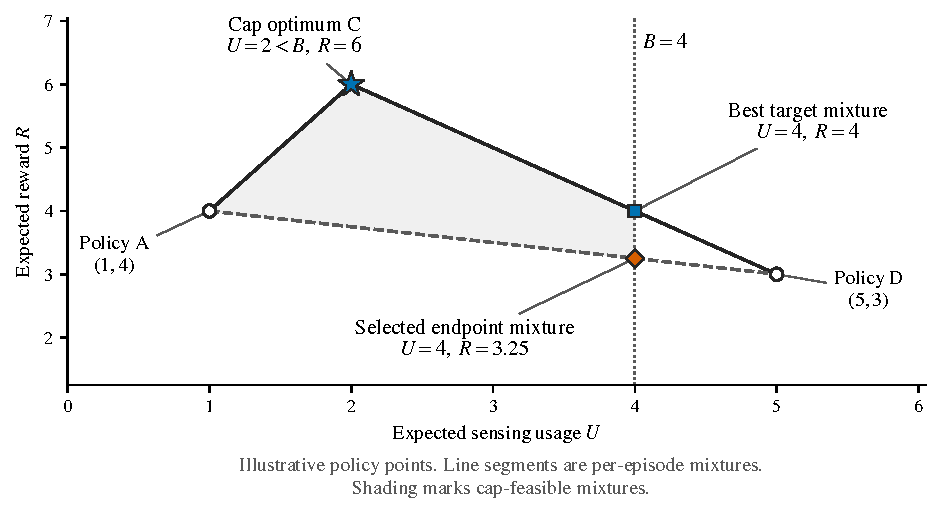
\includegraphics[width=\linewidth]{figures/fig_target_vs_cap.pdf}
\caption{An expected-usage target and a usage cap answer different questions. This schematic uses three illustrative policies and their per-episode mixtures, not benchmark data. The target $U=B$ is the vertical line, while the shaded portion of the mixture hull satisfies the cap $U\le B$. Suppose increasing grid weights select policies C, A, then D, so A and D form the selected crossing pair. A selected endpoint mixture can meet the target yet earn less than another mixture at the same usage. The highest-return cap-feasible policy can also leave part of the budget unused. These possibilities explain why calibration alone supplies neither an equality-constrained nor a cap-constrained reward optimum. They do not assert that every instance has either shortfall.}
\label{fig:target_vs_cap}
\Description{Illustrative policy points in expected usage and return coordinates form a triangle of attainable per-episode mixtures. A vertical budget line intersects two edges at different returns. The lower intersection is the selected endpoint mixture, the higher is the best mixture at that target among the illustrated policies. The highest-return vertex lies strictly left of the budget line and is the cap optimum over these policies and their mixtures.}
\end{figure}

Discrete policy changes produce usage gaps, so a single weight need not attain $B$. The curve may also be nonmonotone. We estimate it on a finite grid and use the following four distinct objects to avoid treating a grid estimate as an exact inverse.

\begin{definition}[Operational shadow price, crossing bracket, and endpoint mixture]
\label{def:pi3}
Fix the usage curve $U(w)$ of the implemented family on $w \ge 0$ and a budget $B$. Four objects are involved, and they are distinct. First, the \emph{level set} $U^{-1}(B) = \{w \ge 0 : U(w) = B\}$ is the set of weights at which usage equals the budget exactly. It is empty when $B$ falls inside a usage gap, and it can be a nondegenerate set when $U$ is flat at level $B$. Second, for a budget that the curve crosses from below, the \emph{crossing threshold} $w^{\dagger}(B)$ is the single weight at which the curve last passes from below $B$ to at or above $B$, namely the supremum of the weights $w$ with $U(w) < B$ that precede a weight with usage at or above $B$. It is undefined for a budget the curve never crosses from below, whether because the curve sits at or above $B$ at every weight, as Tiger's does at $B{=}4$ in Table~\ref{tab:collapse-breadth}, or because it never reaches $B$, and the solver then reports a non-straddling fallback flagged as unbracketed. Under the local non-monotonicity documented in Section~\ref{sec:pi2} the curve can cross $B$ more than once, and taking the last crossing is a convention adopted here, not a property of the problem. At a jump of the curve the threshold is a single number, the location of the jump, even though the level set is empty there. The operational shadow price of this article is this threshold, $w^*(B) := w^{\dagger}(B)$, defined wherever the threshold is. Third, the \emph{crossing bracket} $(w_{\mathrm{lo}}, w_{\mathrm{hi}}]$ is the finite-grid estimate of the threshold that the released solver reports (\texttt{rho\_\allowbreak aif/\allowbreak budget.py}). Its lower endpoint is the largest grid weight with $U(w_{\mathrm{lo}}) < B$ and its upper endpoint is the first subsequent grid weight with $U(w_{\mathrm{hi}}) \geq B$, so the bracket straddles the budget on the grid whenever a grid point at or above $B$ follows the last grid weight with usage below $B$, and its closed enclosure $[w_{\mathrm{lo}}, w_{\mathrm{hi}}]$ contains the threshold whenever the curve has no crossing of $B$ that the grid fails to resolve, between grid weights or beyond the last one (a curve whose final grid point falls back below $B$ would instead yield a non-straddling fallback flagged as such even though its threshold can exist, a shape no swept curve exhibits). The enclosure is stated closed because the threshold can coincide with $w_{\mathrm{lo}}$ itself, when the curve rises immediately after that grid weight, and the half-open reported bracket excludes that one point by construction. The width of the bracket is grid resolution. The weights inside it do not each attain the budget, and the bracket is not a set of exact prices. Offline solving additionally accepts the nearest grid point as achieving the budget when $|U(w) - B| \leq \max(0.3,\, 0.1B)$, a numerical tolerance that affects achievability calls only, never the bracket. Fourth, the \emph{endpoint mixture} is the randomized policy that, when $B$ falls inside a usage gap so that no single weight attains it, plays the policy at $w_{\mathrm{hi}}$ with probability $q = (B - U(w_{\mathrm{lo}}))/(U(w_{\mathrm{hi}}) - U(w_{\mathrm{lo}}))$ and the policy at $w_{\mathrm{lo}}$ otherwise, choosing afresh each episode. By linearity its expected usage is exactly $B$. This is one randomized policy attaining the budget in expectation, not an interval of scalar prices, and it mirrors the classical constrained-MDP fact that optimal budget-constrained policies may need to be randomized \citep{altman1999,kim2011cpomdp}.

A budget is attainable by some per-episode mixture of two members of the family iff $\inf_{w \ge 0} U(w) \le B \le \sup_{w \ge 0} U(w)$, up to the closure of the attainable usage set, since mixing two members whose usages straddle $B$ attains it in expectation. The endpoint mixture of the fourth object attains it only when the budget is straddled by a last crossing from below, that is, when the solver returns a straddling bracket, which holds at every budget for which this article reports a mixture, while the unbracketed cases (Tiger at $B{=}4$ in Table~\ref{tab:collapse-breadth} and the declared-unattainable budgets of Section~\ref{sec:budget_frontier}) are reported as such. A curve that only descends through $B$, with usage $2$ below some weight and $1$ above it and $B{=}1.5$, is attainable by mixing the two plateaus but has no crossing from below, so its crossing bracket and endpoint mixture are undefined and the solver flags the fallback. The lower endpoint need not be $U(0)$. Usage is not monotone in $w$, and the implemented family can spend less at a positive weight than at $w{=}0$ (on Tileworld $6{\times}6$, reward-only Planning at $w{=}0$ scans $15.64$ times per episode while $w{=}1$ scans $14.75$, Section~\ref{sec:tileworld}). Within the suite, $U(0)>0$ reflects instrumental sensing (observing pays for itself on reward alone at some instances) and the upper endpoint reflects belief saturation and the episode step cap.
\end{definition}

\subsection{Exact Scale Equivariance}
\label{sec:pi1}

Let an $\alpha$-rescaled environment multiply every pragmatic quantity, including observation costs, by $\alpha>0$, while leaving dynamics, observations, and belief updates unchanged. Scaling $w$ by the same factor then multiplies every candidate value by $\alpha$.

\begin{proposition}[Exact scale equivariance]
\label{prop:pi1}
For every $\alpha>0$ and $w \ge 0$, the receding-horizon Planning+IG agent facing the $\alpha$-scaled environment with weight $\alpha w$ selects the same action as the agent facing the unscaled environment with weight $w$, at every belief, provided ties are broken by a scale-independent rule. Consequently the closed-loop policies coincide, and so do the induced distributions of every quantity that depends on the actions alone. For usage denominated in observation count this gives
\begin{equation}
\label{eq:pi1}
U_{\mathrm{count},\alpha}(\alpha w) = U_{\mathrm{count}}(w),
\end{equation}
and for usage denominated in cumulative sensing cost, which sums the rescaled costs of the same actions, it gives $U_{\mathrm{cost},\alpha}(\alpha w) = \alpha\, U_{\mathrm{cost}}(w)$.
\end{proposition}

The proof follows by preserving each action ranking and inducting over decision points (Appendix~\ref{app:theory_budget_proofs}). The implementation's comparison tolerance is relative, $10^{-12}$ times the larger candidate magnitude, and favors the incumbent commit action. This rule scales with value. An absolute tolerance would not. Floating-point rounding need not be exactly homogeneous, so bit-identical collapse in the experiments is a measurement rather than a mathematical guarantee.

For count usage, plotting against $w/\alpha$ gives the same curve. Cost usage must also be divided by $\alpha$. Wherever the threshold exists,
\[
w^*_{\mathrm{count}}(B;\alpha)=\alpha w^*_{\mathrm{count}}(B;1),\qquad
w^*_{\mathrm{cost}}(B;\alpha)=\alpha w^*_{\mathrm{cost}}(B/\alpha;1).
\]
The grid bracket rescales only when the grid itself is multiplied by $\alpha$. A fixed $w=1$ at scale $\alpha$ instead behaves as $w=1/\alpha$ at scale 1, with implicit count budget $B_{\mathrm{EFE}}(\alpha):=U(1/\alpha)$. Equivariance applies equally to a directly tuned weight on the correspondingly rescaled grid.

\subsection{Monotone Comparative Statics and the Usage Staircase}
\label{sec:pi2}

Scale equivariance does not imply that usage increases with $w$. The general monotonicity result concerns expected information gain under exact maximization over a fixed plan set.

\begin{proposition}[Monotone comparative statics for exact maximizers]
\label{prop:pi2}
Let $\Pi$ be any fixed set of plans and, for $w \ge 0$, let $\pi_w \in \arg\max_{\pi \in \Pi} R(\pi) + w\, I(\pi)$. Then for $w_2 > w_1 \ge 0$,
\begin{equation}
I(\pi_{w_2}) \ge I(\pi_{w_1}) \quad \text{and} \quad R(\pi_{w_2}) \le R(\pi_{w_1}).
\end{equation}
\end{proposition}

Adding the two optimality inequalities proves the information-gain inequality. Substitution then proves the return inequality (Appendix~\ref{app:theory_budget_proofs}). Neither implies monotone observation count. A policy with fewer, more informative observations can collect more information. Moreover, a receding-horizon agent maximizes again at each reached belief, so its complete trajectory is not a single optimizer over the fixed plan set in the proposition. The empirical usage staircases can therefore dip, as they do on Bandit and Tileworld (Section~\ref{sec:stairs}).

The single observe-or-commit decision does admit an exact usage threshold. We write $w_{\mathrm{thresh}}$ for the $w^*_{\mathrm{thresh}}$ of Proposition~\ref{prop:nearopt}, dropping the star to distinguish it from $w^*(B)$.

\begin{corollary}[Proposition~\ref{prop:nearopt}'s onset thresholds are usage-staircase knots]
\label{cor:pi4}
In the two-state $H{=}1$ setting of Proposition~\ref{prop:nearopt} with $w_{\mathrm{thresh}} \geq 0$, equivalently $c \geq (p - \tfrac{1}{2})(R^+ - R^-)$, for any budget $B \in (0,1)$ the crossing threshold of Definition~\ref{def:pi3} is exactly $w_{\mathrm{thresh}}$, the weight at which the staircase leaves zero, and the closed enclosure $[w_{\mathrm{lo}}, w_{\mathrm{hi}}]$ of a finite-grid crossing bracket contains that threshold whenever the sampled usages straddle $B$, locating it to grid resolution rather than equalling it. When $w_{\mathrm{thresh}} < 0$ every nonnegative weight already observes, so $U \equiv 1$ on $[0,\infty)$ and no onset knot lies in the nonnegative range. The onset boundary of the budgeted problem recovers Proposition~\ref{prop:nearopt}'s closed form as the first knot of the usage staircase.
\end{corollary}

Its proof is the single-step curve $U(w)=\mathbb 1[w>w_{\mathrm{thresh}}]$ under the commit-favoring tie rule. The full argument and implementation check are in Appendix~\ref{app:theory_budget_proofs}. That check runs whole receding-horizon episodes and verifies the onset, not a claim that every such episode takes exactly one observation.

\subsection{Solving for the Shadow Price}
\label{sec:budget_solve}

We estimate $U(w)$ by multi-seed Monte Carlo on a log-spaced grid: five seeds and 100 episodes per cell on the discrete observe-then-commit domains, 40 on Tileworld-$6\times6$, and lighter settings on tree-search domains (Section~\ref{sec:budget_experiments}). Per-seed means give standard errors. We report the crossing bracket and the grid weight $\hat w(B)$ minimizing $|U-B|$, rather than a bisection root. This plotted point can lie on the lower bracket edge or, at a slack budget, below it. Count and cost usage are distinct. They differ by a fixed conversion only when all sensing actions share a cost (Section~\ref{sec:cost_budget}).

\subsection{Online Dual Control of the Shadow Price}
\label{sec:pi5}

A reward-scale change moves the count-budget crossing. To adjust without a fresh grid sweep, we adapt SAC's automatic temperature update \citep{haarnoja2018sac}, replacing the policy-entropy target by a sensing target. After episode $t$ with observed usage $U_t$, update
\begin{equation}
\label{eq:dual_update}
w_{t+1}=\mathrm{Proj}_{[0,w_{\max}]}\big(w_t+a_t(B-U_t)\big),\qquad a_t=\frac{\eta_0}{1+\delta t},
\end{equation}
where $\eta_0$ is the initial step, $\delta$ its decay rate, and projection clips the weight to $[0,w_{\max}]$. If $\mathbb E[U_t\mid w_t]=U(w_t)$, usage is a noisy observation of the curve. Underspending raises $w$ and overspending lowers it. This sign corrects usage only under suitable crossing conditions.

The proposition covers the projected decaying-step controller, with finite $w_{\max}$ and $\delta>0$. Every reported run uses $w_{\max}=100$ and $\delta=0.02$. No iterate exceeded 3.1, so the upper projection was present but inactive. It does not cover the released library default, which has a constant step and no upper projection, or the reset-on-shift heuristic described below.

\begin{proposition}[Stationary convergence of the dual controller]
\label{prop:pi5}
Consider the projected decaying-step controller, the recursion~\eqref{eq:dual_update} with a finite $w_{\max}$ and step sizes satisfying $\sum_t a_t = \infty$ and $\sum_t a_t^2 < \infty$ (the schedule in~\eqref{eq:dual_update} with $\delta>0$). Suppose four conditions hold. (i) The environment, agent family, and budget $B$ are stationary, so that $\mathbb{E}[U_t \mid w_t] = U(w_t)$ for a fixed function $U$. (ii) Per-episode usage is bounded, which holds here because usage is bounded by the episode step cap, and each episode is run on an environment reset and freshly seeded independently of the past, so that the noise $U_t - U(w_t)$ is a martingale difference with bounded conditional second moment. (iii) There is a single crossing $w^* \in (0, w_{\max})$ with $U(w) < B$ for $w < w^*$ and $U(w) > B$ for $w > w^*$. (iv) The curve stays away from the budget outside every neighborhood of the crossing, that is, for every $0 < \epsilon_1 < \epsilon_2$, $\inf\{\,|U(w) - B| : \epsilon_1 \le |w - w^*| \le \epsilon_2,\ w \in [0, w_{\max}]\,\} > 0$. Then $w_t \to w^*$ with probability one, and hence in probability. Condition (iii) does not require $U(w^*) = B$, and condition (iv) does not require continuity, so the conclusion covers a gap budget in the sense of Definition~\ref{def:pi3}, where $U$ jumps over $B$ at $w^*$ without touching it. What converges in that case is the weight. The usage at the limit is $U(w^*)$, one side of the jump, so the expected usage at $w_t$ need not converge to $B$. The running average of observed usage under the schedule in~\eqref{eq:dual_update} does converge to $B$, $\frac{1}{n}\sum_{t<n} U_t \to B$ with probability one, gap budgets included, as Appendix~\ref{app:theory_controller} proves. Attaining $B$ in expectation with one stationary policy at a gap budget is the job of the endpoint mixture of Definition~\ref{def:pi3}, not of this recursion.
\end{proposition}

The update is a projected Robbins--Monro recursion \citep{robbins1951}, with classical almost-sure extensions due to \citet{blum1954} and constrained treatments in \citet{kushner1978}. Appendix~\ref{app:theory_controller} proves this bounded scalar case directly by a supermartingale argument, including discontinuous curves. Kronecker's lemma gives the running-average result for the harmonic schedule above. The theorem is conditional on one sign-consistent crossing and does not cover an arbitrary nonmonotone usage curve.

The reset-on-shift variant detects a persistent recent usage mismatch once the step size has fallen below half its initial value, then restarts the decay clock at zero. These resets break the single diminishing-step schedule, so the proposition does not justify their convergence. Section~\ref{sec:dual_multiseed} evaluates both decay-only and reset-on-shift recovery empirically. Constant-step tracking would require separate drift and noise arguments and is not claimed here.

\subsection{Positioning against Prior Art}
\label{sec:budget_positioning}

Adjusting a price to meet a resource target is classical in constrained MDPs \citep{altman1999}, rational inattention \citep{sims2003,matejka2015}, and SAC \citep{haarnoja2018sac}. Our contribution is its operational use for sensing within the Planning+IG family, with separate count and cost equivariance, finite-grid crossing estimates, endpoint mixtures, and a conditional online convergence result. Rational inattention constrains information processing. Here the design input is sensing usage, while $w$ prices information gain.

An exact constrained-POMDP solver can randomize belief-dependently and outperform a family that runs one weight throughout each episode \citep{kim2011cpomdp}. Our endpoint mixture only randomizes that weight between episodes. The references in Section~\ref{sec:cpomdp} are mixtures selected as cap-feasible from simulated usage estimates for policies in a SARSOP usage-penalty sweep. They are not certified constrained optima. Sampling error and selection over noisy estimates qualify all measured reference gaps. The shallow RockSample reference fails to reach EFE's operating region. Appendix~\ref{app:theory_positioning} reports that limitation rather than treating it as optimality evidence.

Sequential Bayesian experimental design selects tests for information gain about a latent parameter \citep{lindley1956,foster2021dad}. Here reward and sensing cost remain in the objective. Reward at the calibrated weight is measured rather than optimized by the usage calibration. The large-weight limit prioritizes information gain. Closely related work gives a Bethe-Lagrangian account of EFE with an internal information constraint \citep{kouw2026bethe}, and recursive per-node dual ascent inside constrained POMDP tree search \citep{stocco2024recursive}. These differ from controlling one information weight across episodes toward a sensing target. Appendix~\ref{app:theory_positioning} develops the comparisons.

Offline calibration does not save the sampling needed for a weight sweep. Its benefit is a design requirement expressed in observable sensing units. Under its hypotheses, the online controller can locate a crossing from interaction without that sweep. Scale equivariance transfers both calibrated and directly tuned weights across pure reward-and-cost rescalings, so transfer is not a unique advantage of budget calibration.
